\usepackage{array}
\usepackage{tikz}
\usetikzlibrary{arrows.meta}
\usepackage{listings}
\lstloadlanguages{Java,Python,HTML,XML,bash,SQL}

% Named colors for literate replacements (avoid ! in \lstset literals).
\colorlet{lstkw}{blue!70!black}
\colorlet{lstkwii}{violet!75!black}
\colorlet{lstflag}{teal!70!black}
\colorlet{lststr}{orange!85!black}
\colorlet{lsthdr}{blue!70!black}
\colorlet{lstcmt}{black!55}

% Shared framed block style.
\lstdefinestyle{mcpblock}{%
  basicstyle=\ttfamily\footnotesize,
  keywordstyle=\bfseries\color{lstkw},
  commentstyle=\itshape\color{lstcmt},
  stringstyle=\color{lststr},
  columns=fullflexible,
  keepspaces=true,
  tabsize=2,
  showstringspaces=false,
  breaklines=true,
  breakatwhitespace=true,
  frame=single,
  rulecolor=\color{black!35},
  backgroundcolor=\color{black!4},
  xleftmargin=0.5em,
  xrightmargin=0.5em,
  aboveskip=4pt,
  belowskip=4pt,
}

% --- JSON (block only) ---
\lstdefinestyle{json}{%
  style=mcpblock,
  morestring=[b]",%
  morecomment=[l]{//},%
  morekeywords={true,false,null},%
  morekeywords=[2]{jsonrpc,method,params,result,id,error},%
  keywordstyle=\bfseries\color{lstkw},
  keywordstyle=[2]\color{lstkwii},
  stringstyle=\color{lststr},
}

% --- TOML (block only) ---
\lstdefinestyle{toml}{%
  style=mcpblock,
  alsoletter={-.*},%
  morestring=[b]",%
  morecomment=[l]\#,%
  morekeywords={true,false},%
  moredelim=[is][\bfseries\color{lsthdr}]{[}{]},%
  keywordstyle=\bfseries\color{lstkw},
  stringstyle=\color{lststr},
}

% --- Bash / shell ---
\lstdefinestyle{bash}{%
  style=mcpblock,
  language=bash,
  morekeywords={npx,npm,uvx,pip,uv,python,node,curl,git,docker,run,ng},%
  morekeywords=[2]{-y,-m,-f,-v,-h,-p,--help,--directory,--version},%
  keywordstyle=\color{lstkwii},
  keywordstyle=[2]\color{lstflag},
  commentstyle=\color{lstcmt},
  stringstyle=\color{lststr},
  literate={@}{{\textcolor{lststr}{@}}}1,
}
\lstdefinestyle{bashinline}{%
  language=bash,
  basicstyle=\ttfamily\small,
  morekeywords={npx,npm,uvx,pip,uv,python,node,curl,git,docker,run,ng},%
  morekeywords=[2]{-y,-m,-f,-v,-h,-p,--help,--directory,--version},%
  keywordstyle=\color{lstkwii},
  keywordstyle=[2]\color{lstflag},
  commentstyle=\color{lstcmt},
  stringstyle=\color{lststr},
  columns=fullflexible,
  keepspaces=true,
  showstringspaces=false,
}

% --- Python ---
\lstdefinestyle{python}{%
  style=mcpblock,
  language=Python,
}
\lstdefinestyle{pythoninline}{%
  language=Python,
  basicstyle=\ttfamily\small,
  keywordstyle=\bfseries\color{lstkw},
  commentstyle=\itshape\color{lstcmt},
  stringstyle=\color{lststr},
  columns=fullflexible,
  keepspaces=true,
  showstringspaces=false,
}

% --- Java ---
\lstdefinestyle{java}{%
  style=mcpblock,
  language=Java,
}
\lstdefinestyle{javainline}{%
  language=Java,
  basicstyle=\ttfamily\small,
  keywordstyle=\bfseries\color{lstkw},
  commentstyle=\itshape\color{lstcmt},
  stringstyle=\color{lststr},
  columns=fullflexible,
  keepspaces=true,
  showstringspaces=false,
}

% Default for bare \lstinline|...| (mostly Java in cs-a); REST blocks use explicit [style=...].
\lstset{style=javainline}

% --- JavaScript (keywords on the style; no custom language name) ---
\lstdefinestyle{js}{%
  style=mcpblock,
  sensitive=true,%
  morecomment=[l]{//},%
  morecomment=[s]{/*}{*/},%
  morestring=[b]',%
  morestring=[b]",%
  morekeywords={%
    break,case,catch,class,const,continue,debugger,default,delete,do,else,%
    export,extends,false,finally,for,function,if,import,in,instanceof,new,%
    null,return,super,switch,this,throw,true,try,typeof,var,void,while,%
    let,static,async,await,of,yield},%
}
\lstdefinestyle{jsinline}{%
  basicstyle=\ttfamily\small,
  keywordstyle=\bfseries\color{lstkw},
  commentstyle=\itshape\color{lstcmt},
  stringstyle=\color{lststr},
  columns=fullflexible,
  keepspaces=true,
  showstringspaces=false,
  sensitive=true,%
  morecomment=[l]{//},%
  morecomment=[s]{/*}{*/},%
  morestring=[b]',%
  morestring=[b]",%
  morekeywords={%
    break,case,catch,class,const,continue,debugger,default,delete,do,else,%
    export,extends,false,finally,for,function,if,import,in,instanceof,new,%
    null,return,super,switch,this,throw,true,try,typeof,var,void,while,%
    let,static,async,await,of,yield},%
}

% --- TypeScript (JavaScript keywords + extras on the style) ---
\lstdefinestyle{ts}{%
  style=js,
  morekeywords={%
    interface,type,implements,private,public,protected,readonly,enum,%
    namespace,abstract,as,is,any,unknown,never,keyof,infer,%
    Component,NgModule,Injectable,Input,Output,Directive,Pipe,%
    inject,standalone,selector,template,templateUrl,styleUrls,%
    providers,imports,declarations,bootstrap},%
  alsoletter={@\$},%
}
\lstdefinestyle{tsinline}{%
  style=jsinline,
  morekeywords={%
    interface,type,implements,private,public,protected,readonly,enum,%
    namespace,abstract,as,is,any,unknown,never,keyof,infer,%
    Component,NgModule,Injectable,Input,Output,Directive,Pipe,%
    inject,standalone,selector,template,templateUrl,styleUrls,%
    providers,imports,declarations,bootstrap},%
  alsoletter={@\$},%
}

% --- SQL ---
\lstdefinestyle{sql}{%
  style=mcpblock,
  language=SQL,
}
\lstdefinestyle{sqlinline}{%
  language=SQL,
  basicstyle=\ttfamily\small,
  keywordstyle=\bfseries\color{lstkw},
  commentstyle=\itshape\color{lstcmt},
  stringstyle=\color{lststr},
  columns=fullflexible,
  keepspaces=true,
  showstringspaces=false,
}

% --- AP CSP pseudocode ---
\lstdefinestyle{pseudo}{%
  style=mcpblock,
  numbers=left,
  numberstyle=\scriptsize\color{lstcmt},
  numbersep=7pt,
  morekeywords={%
    PROCEDURE,REPEAT,UNTIL,TIMES,IF,ELSE,RETURN,DISPLAY,%
    LENGTH,RANDOM,MOVE_FORWARD,ROTATE_LEFT,MOVE_BACKWARD,ROTATE_RIGHT,%
    REMOVE,FOR,TO,WHILE,EACH,IN,APPEND,IsFound,CAN_MOVE,GoalReached,%
    AND,OR,NOT,true,false,min,max,MIN,MAX%
  },
  sensitive=false,
}
\lstdefinestyle{pseudoinline}{%
  basicstyle=\ttfamily\small,
  keywordstyle=\bfseries\color{lstkw},
  commentstyle=\itshape\color{lstcmt},
  columns=fullflexible,
  keepspaces=true,
  showstringspaces=false,
  morekeywords={%
    PROCEDURE,REPEAT,UNTIL,TIMES,IF,ELSE,RETURN,DISPLAY,%
    LENGTH,RANDOM,MOVE_FORWARD,ROTATE_LEFT,MOVE_BACKWARD,ROTATE_RIGHT,%
    REMOVE,FOR,TO,WHILE,EACH,IN,APPEND,IsFound,CAN_MOVE,GoalReached,%
    AND,OR,NOT,true,false,min,max,MIN,MAX%
  },
  sensitive=false,
}

% --- HTML / XML / CSS ---
\lstdefinestyle{html}{%
  style=mcpblock,
  language=HTML,
}
\lstdefinestyle{htmlinline}{%
  language=HTML,
  basicstyle=\ttfamily\small,
  keywordstyle=\bfseries\color{lstkw},
  commentstyle=\itshape\color{lstcmt},
  stringstyle=\color{lststr},
  columns=fullflexible,
  keepspaces=true,
  showstringspaces=false,
}
\lstdefinestyle{xml}{%
  style=mcpblock,
  language=XML,
  numbers=none,
  tabsize=4,
}
\lstdefinestyle{css}{%
  style=mcpblock,
  morekeywords={%
    color,background,background-color,margin,padding,border,border-width,%
    border-style,border-color,width,height,display,font,font-size,font-style,%
    font-weight,text-align,text-decoration,box-sizing,position,overflow,%
    opacity,max-width,min-width,flex,align-items,justify-content,gap,z-index},%
  morecomment=[s]{/*}{*/},%
  morestring=[b]',%
  sensitive=false,
}
\lstdefinestyle{cssinline}{%
  basicstyle=\ttfamily\small,
  keywordstyle=\bfseries\color{lstkw},
  commentstyle=\itshape\color{lstcmt},
  stringstyle=\color{lststr},
  columns=fullflexible,
  keepspaces=true,
  showstringspaces=false,
  morekeywords={%
    color,background,background-color,margin,padding,border,border-width,%
    border-style,border-color,width,height,display,font,font-size,font-style,%
    font-weight,text-align,text-decoration,box-sizing,position,overflow,%
    opacity,max-width,min-width,flex,align-items,justify-content,gap,z-index},%
  morecomment=[s]{/*}{*/},%
  morestring=[b]',%
  sensitive=false,
}

% --- HTTP trace (block only) ---
\lstdefinestyle{http}{%
  basicstyle=\ttfamily\footnotesize,
  alsoletter={-./},%
  morekeywords={GET,POST,PUT,DELETE,PATCH,HTTP,OK,Accepted,No,Found,Bad,Unauthorized,Conflict,Request},%
  morekeywords=[2]{Host,Accept,Content-Type,event,data},%
  keywordstyle=\bfseries\color{lstkwii},
  keywordstyle=[2]\color{lsthdr},
  frame=single,
  framerule=0.4pt,
  rulecolor=\color{black!35},
  backgroundcolor=\color{black!4},
  framesep=3pt,
  xleftmargin=2pt,
  xrightmargin=2pt,
  breaklines=true,
  breakatwhitespace=true,
  columns=fullflexible,
  keepspaces=true,
  showstringspaces=false,
  aboveskip=4pt,
  belowskip=4pt,
}

% Side-by-side request/response (\texttt{cs-web/rest.tex}).
\tikzset{%
  http@arrow/.style={%
    -{Stealth[scale=0.88]}, semithick, shorten >=0.5pt, shorten <=0.5pt, draw=black!55},
}
\newenvironment{httpexchange}{%
  \par\addvspace{\baselineskip}%
  \begingroup
  \hfuzz=30pt\relax
  \begin{center}%
  \noindent
  \begin{tabular}{@{} m{0.4\linewidth} >{\centering\arraybackslash}m{1.28cm} m{0.4\linewidth} @{}}%
}{%
  \end{tabular}%
  \end{center}%
  \endgroup
  \par\addvspace{\baselineskip}%
}
\newcommand{\httpmidarrows}{%
  &
  \begin{minipage}[c]{1.28cm}%
    \centering
    \normalfont\footnotesize REQ\par\vspace{1pt}%
    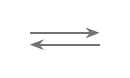
\begin{tikzpicture}[x=1cm, y=0.75cm]
      \draw[http@arrow] (0,0.1) -- (0.92,0.1);
      \draw[http@arrow] (0.92,-0.1) -- (0,-0.1);
    \end{tikzpicture}\par\vspace{1pt}%
    \normalfont\footnotesize RESP%
  \end{minipage}%
  &
}
